\chapter*{La route Puno – Cusco\markboth{La route Puno – Cusco}{}}
\section*{22 mai 2015}
5 jours de vélo pour aller de Puno au bord du lac Titicaca à Cusco.

 Un petit détour pour visiter le village de Lampa. 

 

\begin{center} 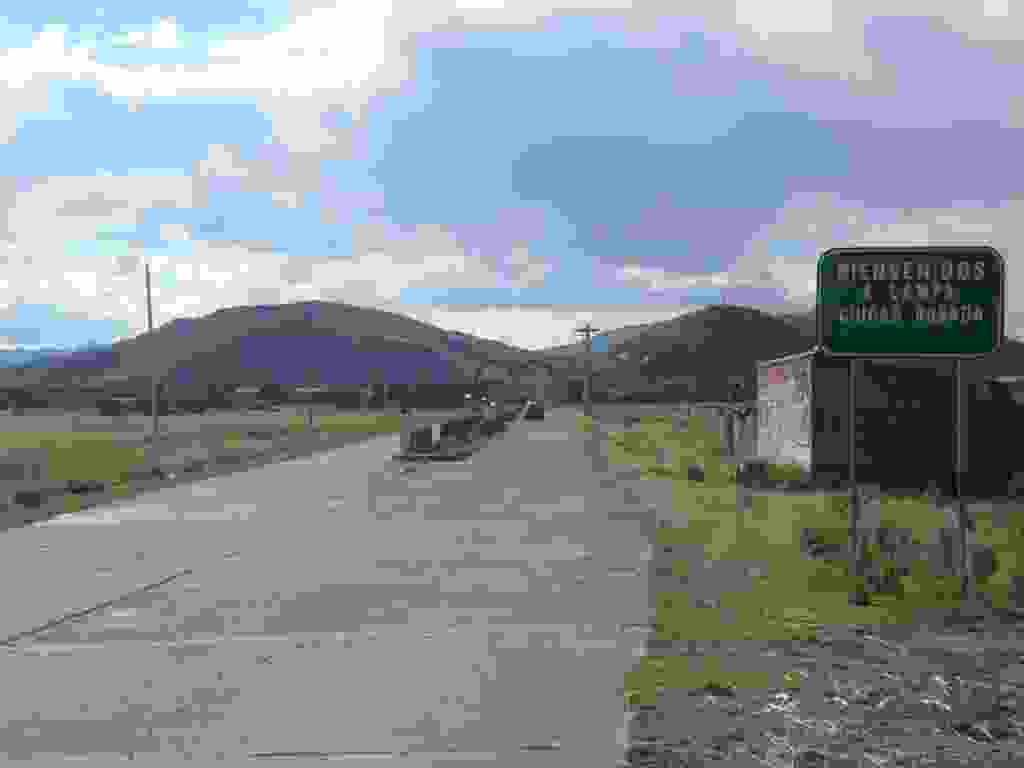
\includegraphics[width=\mywidth]{../wp-content/uploads/2015/05/P5124011-1024x768.jpg} \end{center}

 

 Très belle église, construite par les espagnols sur des fondations incas, comme beaucoup au Pérou. 

 

\begin{center} 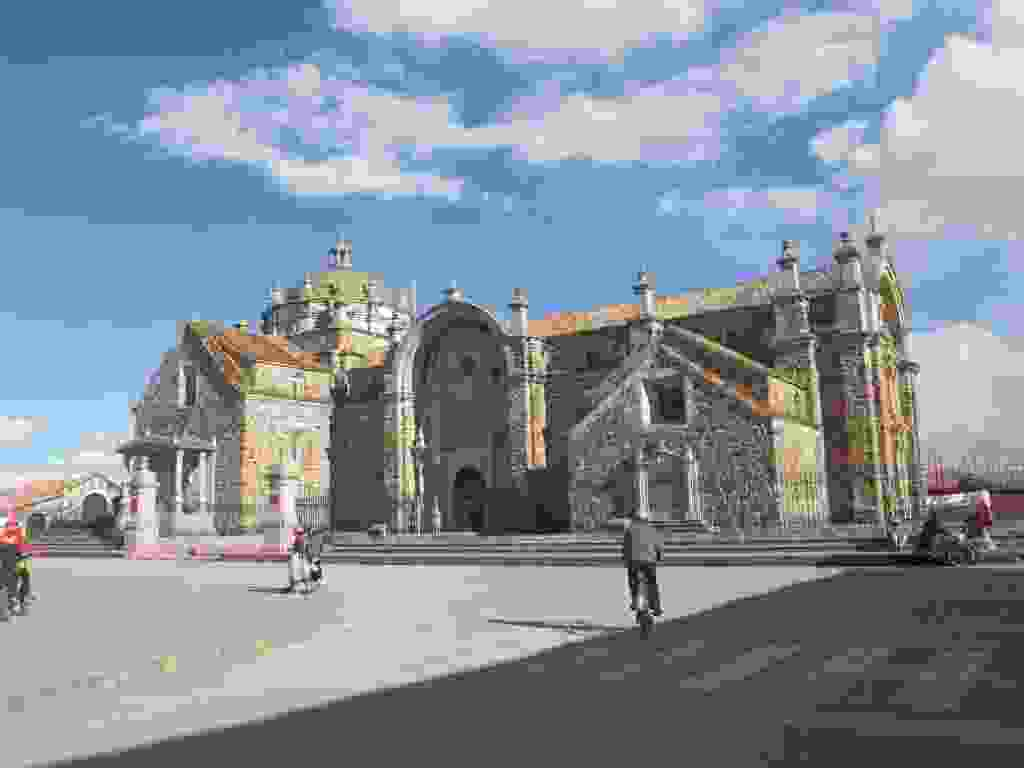
\includegraphics[width=\mywidth]{../wp-content/uploads/2015/05/P5124012-1024x768.jpg} \end{center}

 

 Les catacombes d´origine inca. 

 

\begin{center} 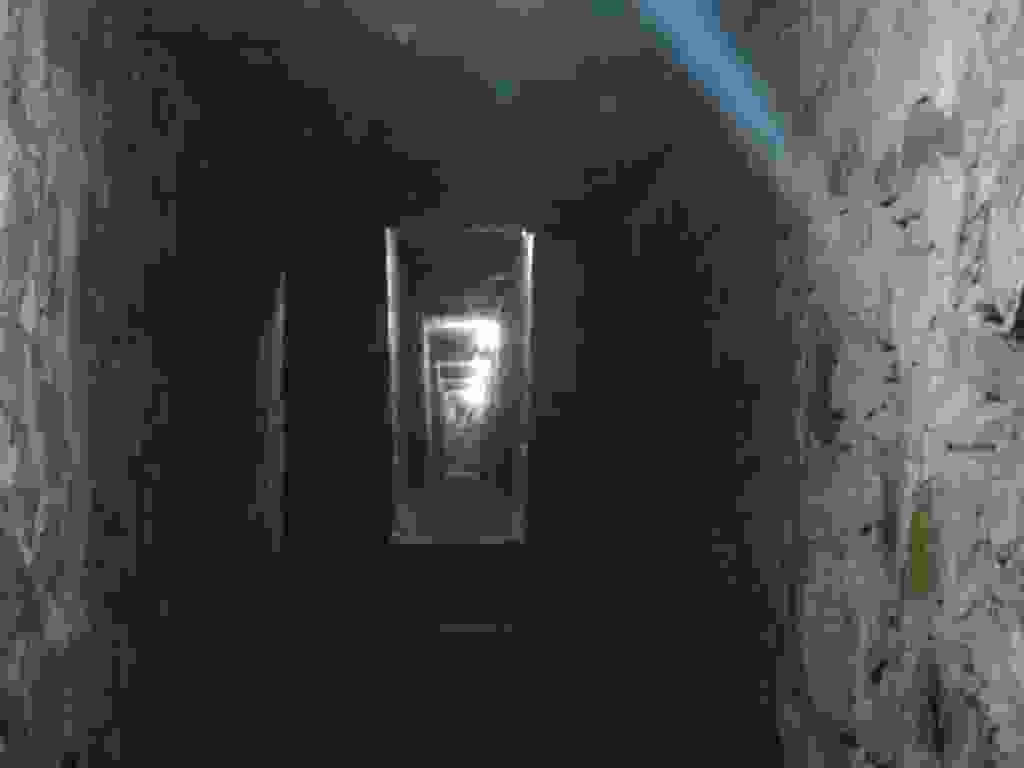
\includegraphics[width=\mywidth]{../wp-content/uploads/2015/05/P5124020-1024x768.jpg} \end{center}

 

 L´église contient une reproduction de la sculture La Pietà de Michel-Ange. 

 

\begin{center} 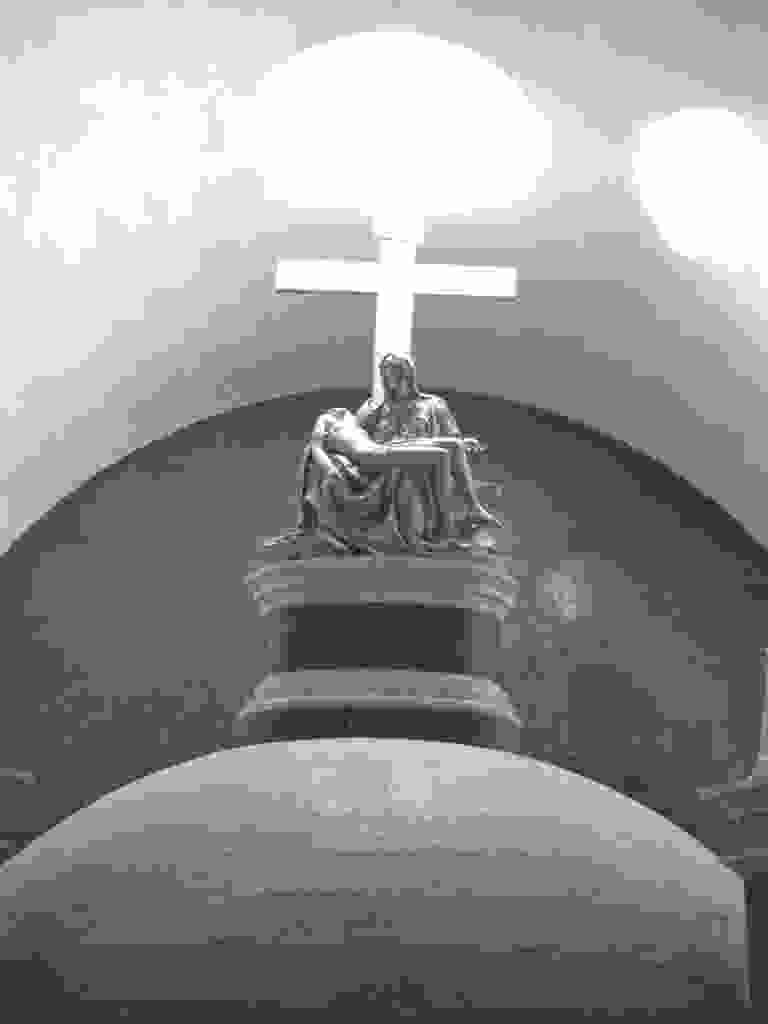
\includegraphics[width=\mywidth]{../wp-content/uploads/2015/05/P5124022-768x1024.jpg} \end{center}

 

 La route traverse de belles vallées et on aperçoit parfois des sommets enneigés. 

 

\begin{center} 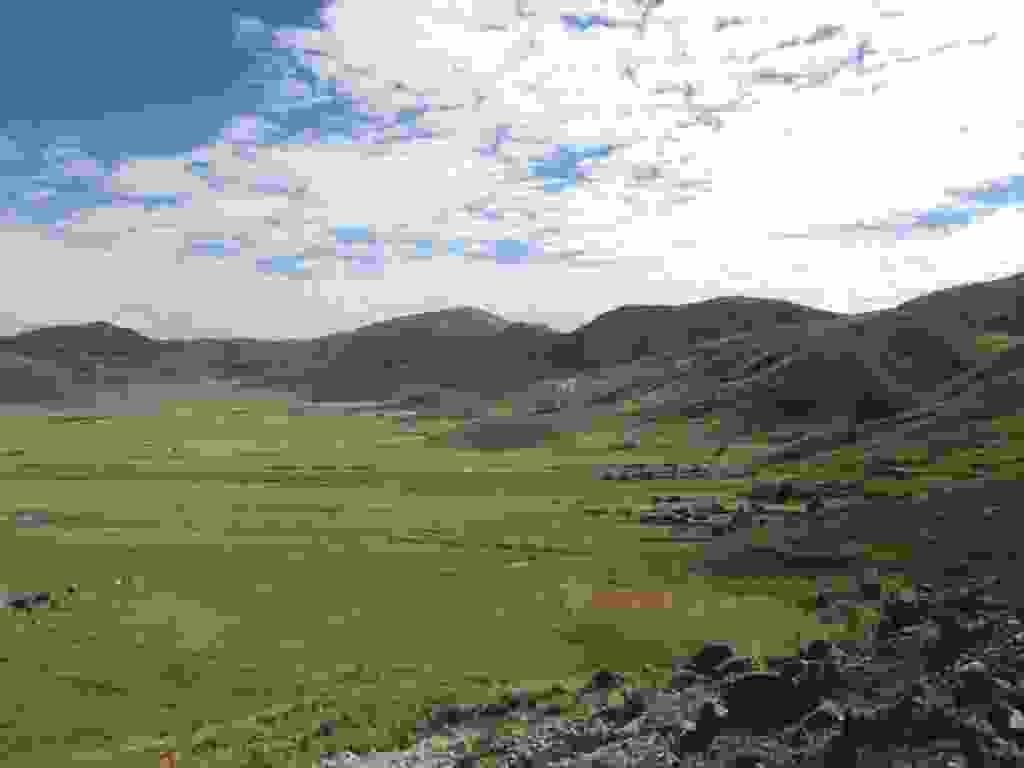
\includegraphics[width=\mywidth]{../wp-content/uploads/2015/05/P5134030-1024x768.jpg} \end{center}

 

 

\begin{center} 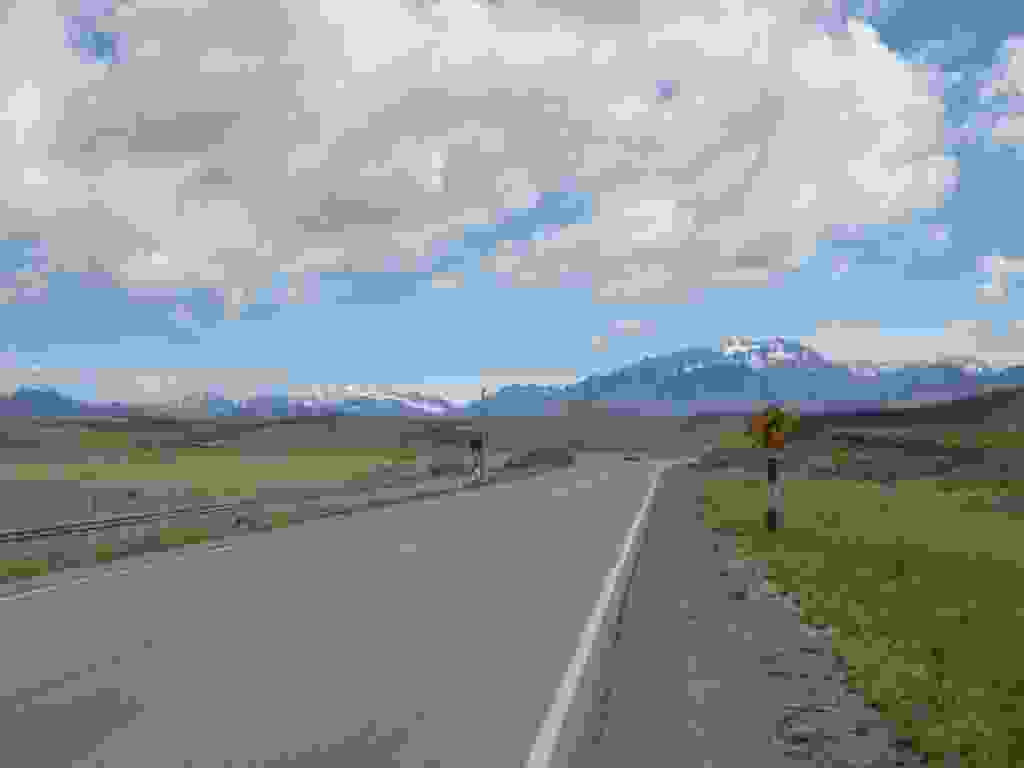
\includegraphics[width=\mywidth]{../wp-content/uploads/2015/05/P5144046-1024x768.jpg} \end{center}

 

 

\begin{center} 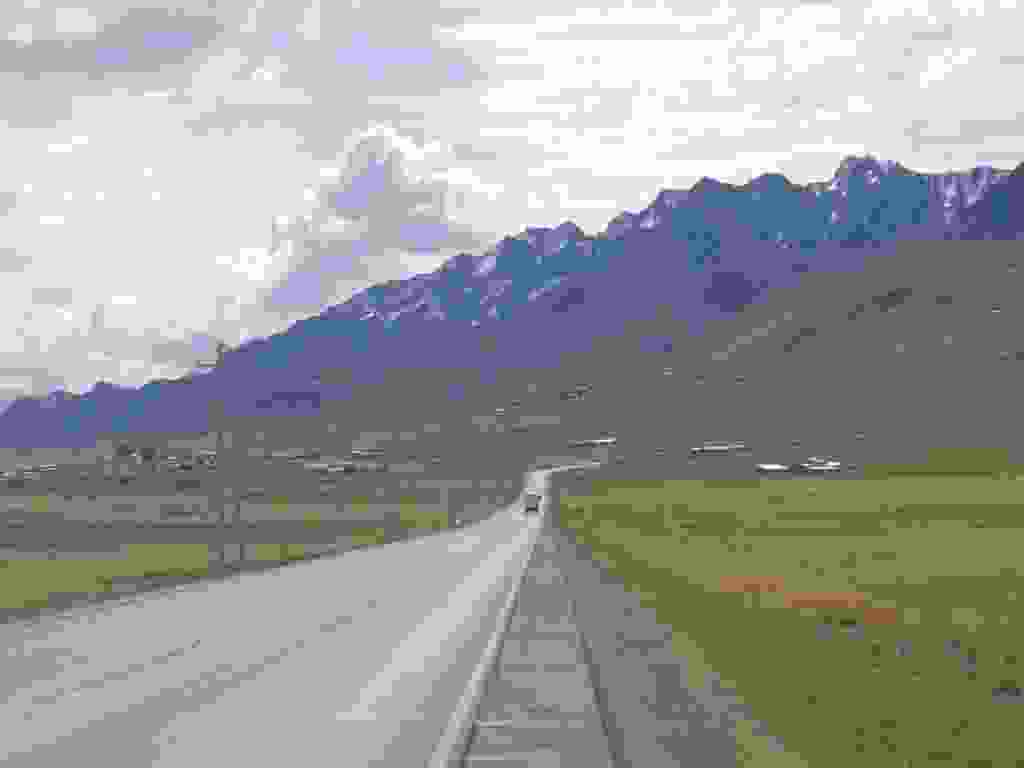
\includegraphics[width=\mywidth]{../wp-content/uploads/2015/05/P5144050-1024x768.jpg} \end{center}

 

 Le point le plus haut de la route : col de La Raya à 4300m. 

 

\begin{center} 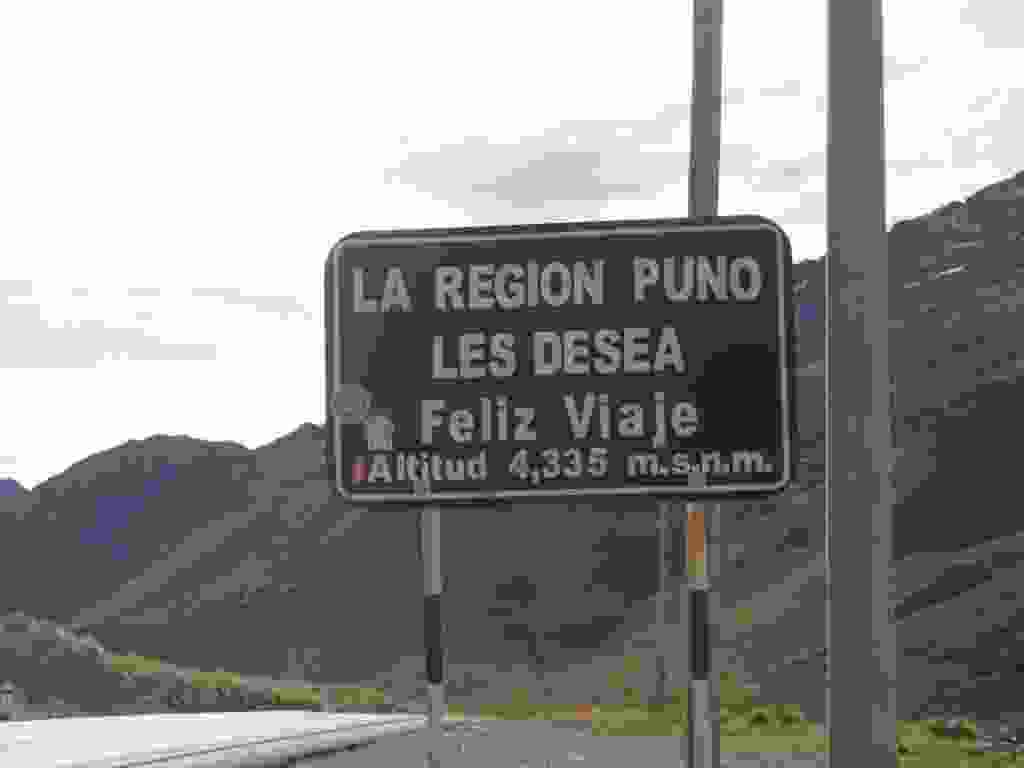
\includegraphics[width=\mywidth]{../wp-content/uploads/2015/05/P5144056-1024x768.jpg} \end{center}

 

 

\begin{center} 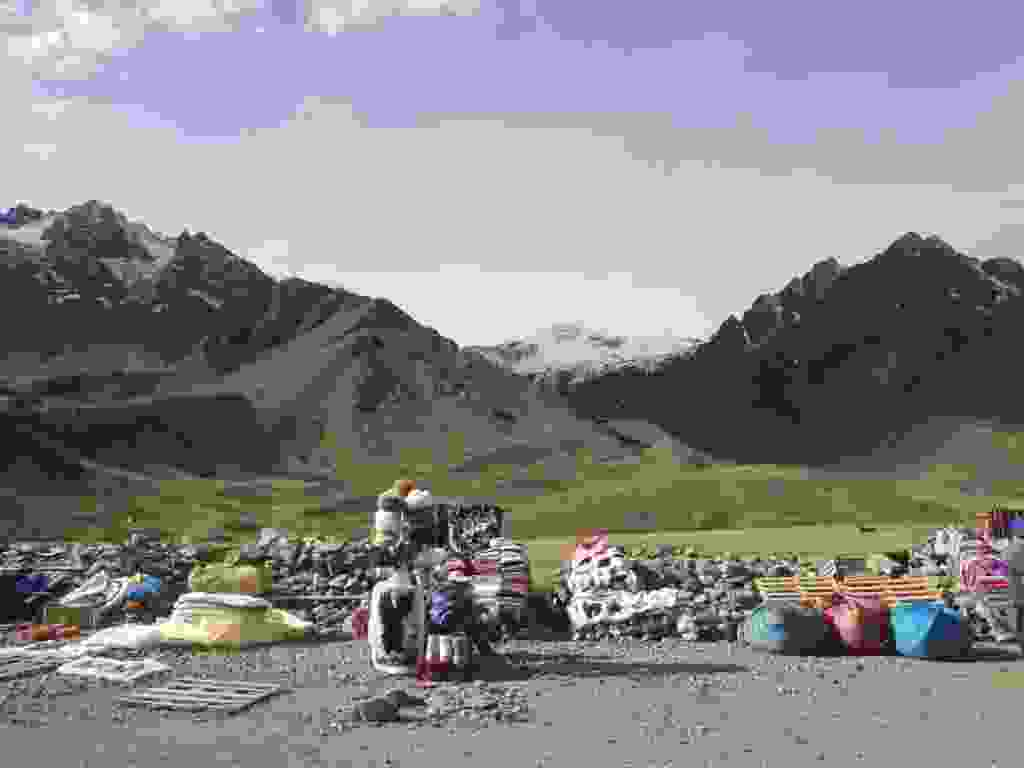
\includegraphics[width=\mywidth]{../wp-content/uploads/2015/05/P5144054-1024x768.jpg} \end{center}

 

 Bivouac dans la descente. 

 

\begin{center} 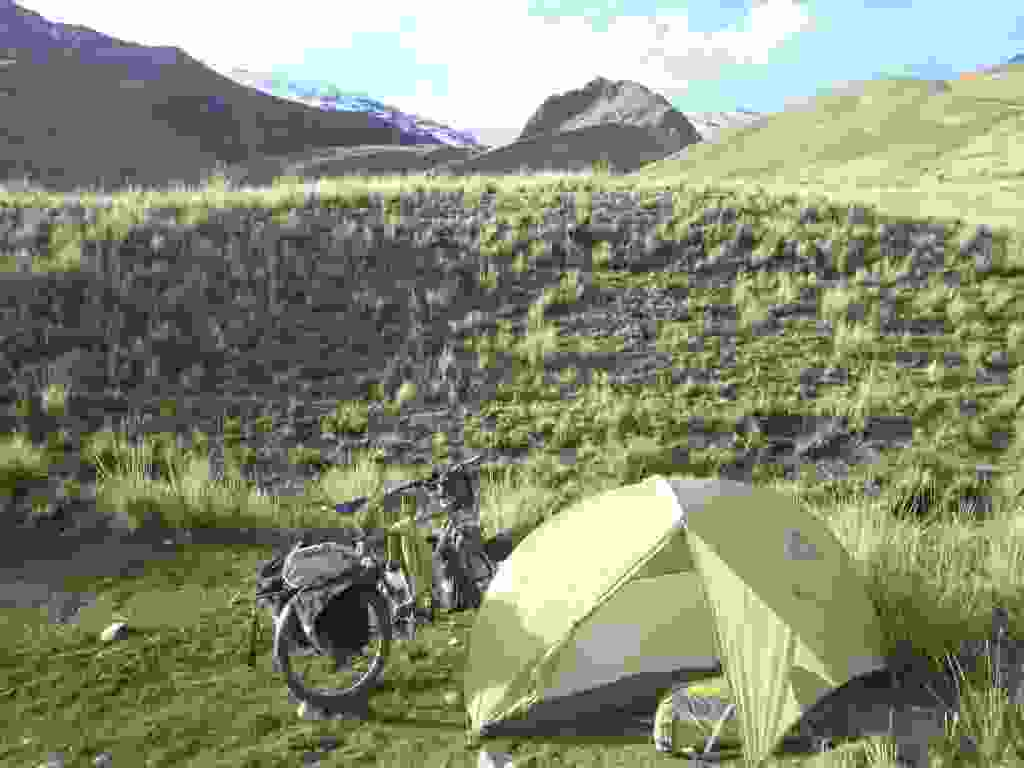
\includegraphics[width=\mywidth]{../wp-content/uploads/2015/05/P5144064-1024x768.jpg} \end{center}

 

 Le matin je me réveille avec un troupeau de lamas et alpagas juste au dessus de moi. 

 

\begin{center} 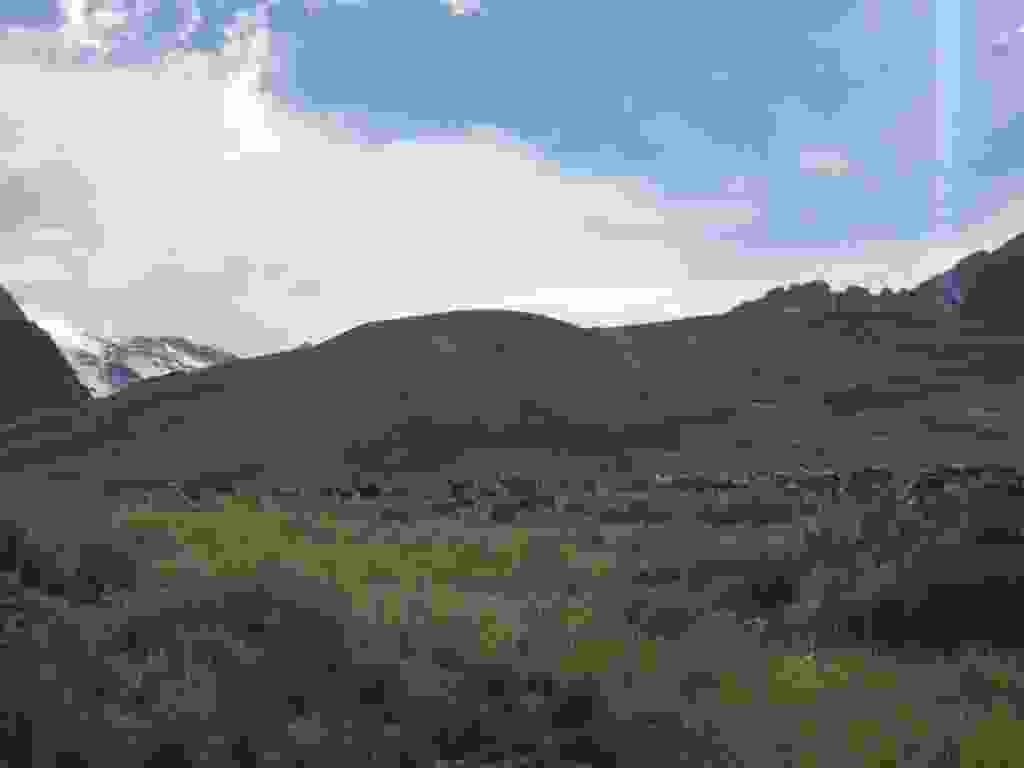
\includegraphics[width=\mywidth]{../wp-content/uploads/2015/05/P5154068-1024x768.jpg} \end{center}

 

 Sur la route beaucoup de petits restaurants où on peut manger un bon repas avec une soupe et un plat pour à peine 1,5€. 

 

\begin{center} 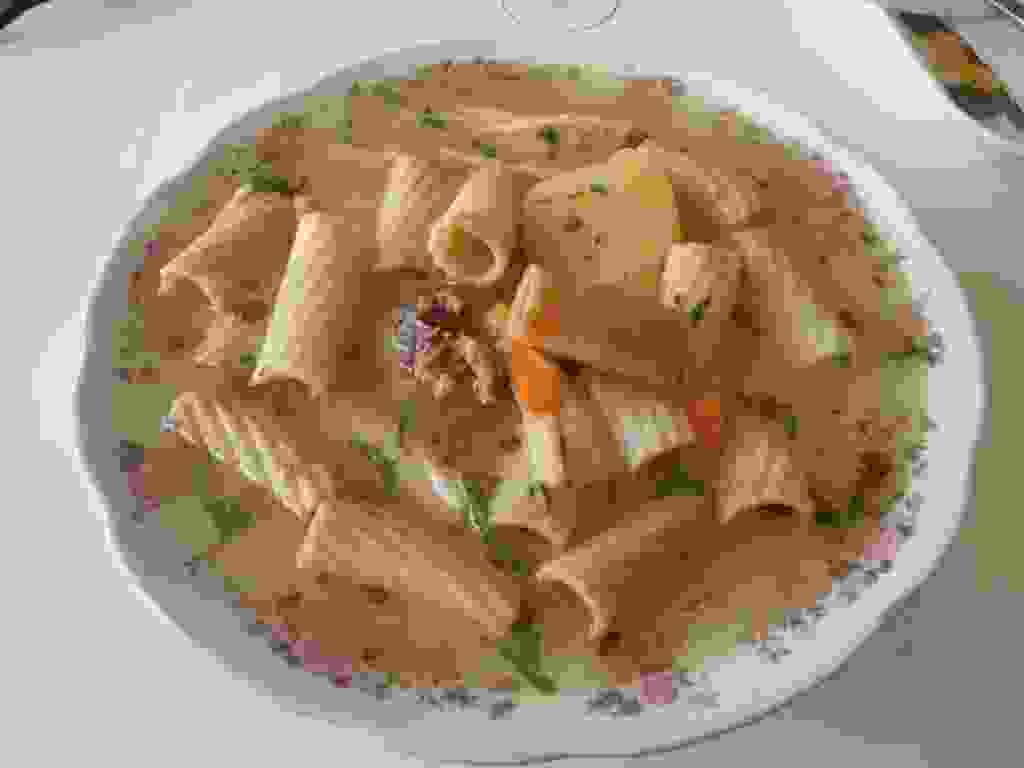
\includegraphics[width=\mywidth]{../wp-content/uploads/2015/05/P5134037-1024x768.jpg} \end{center}

 

 

\begin{center} 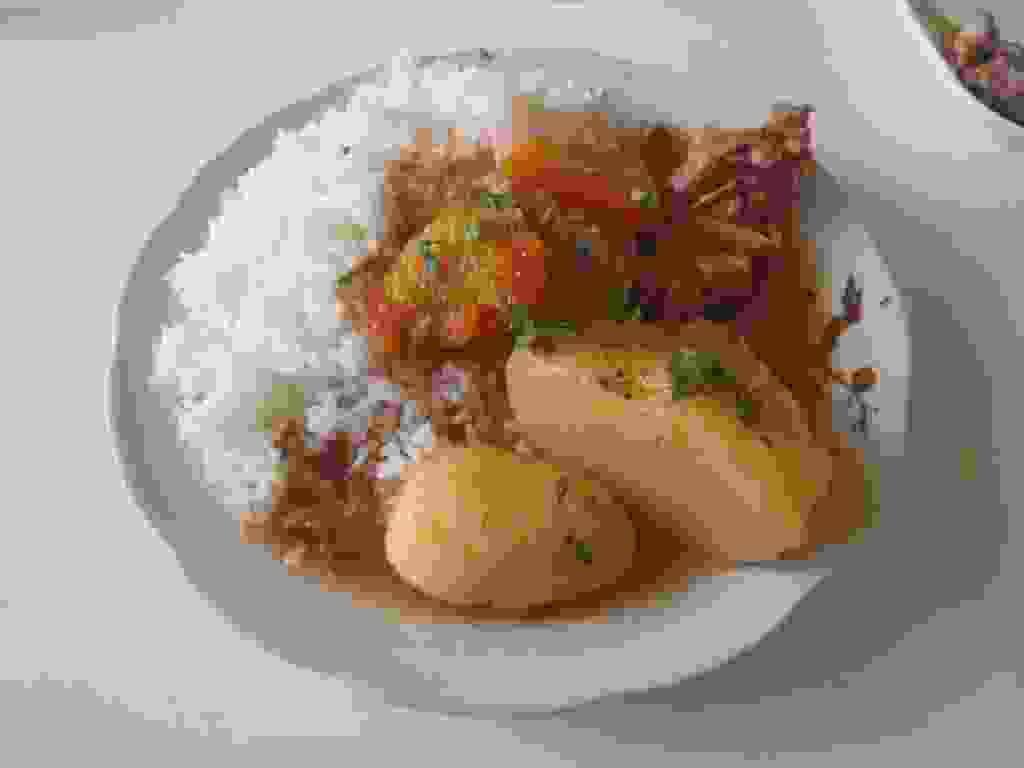
\includegraphics[width=\mywidth]{../wp-content/uploads/2015/05/P5134038-1024x768.jpg} \end{center}

 

 Avant d´arriver à Cusco, plusieurs sites archéologiques à visiter.

 Le site de Rachqi, situé sur le chemin de l´inca, avec les restes d´un temple, d´habitations et de batiments de stockage de nourriture. 

 

\begin{center} 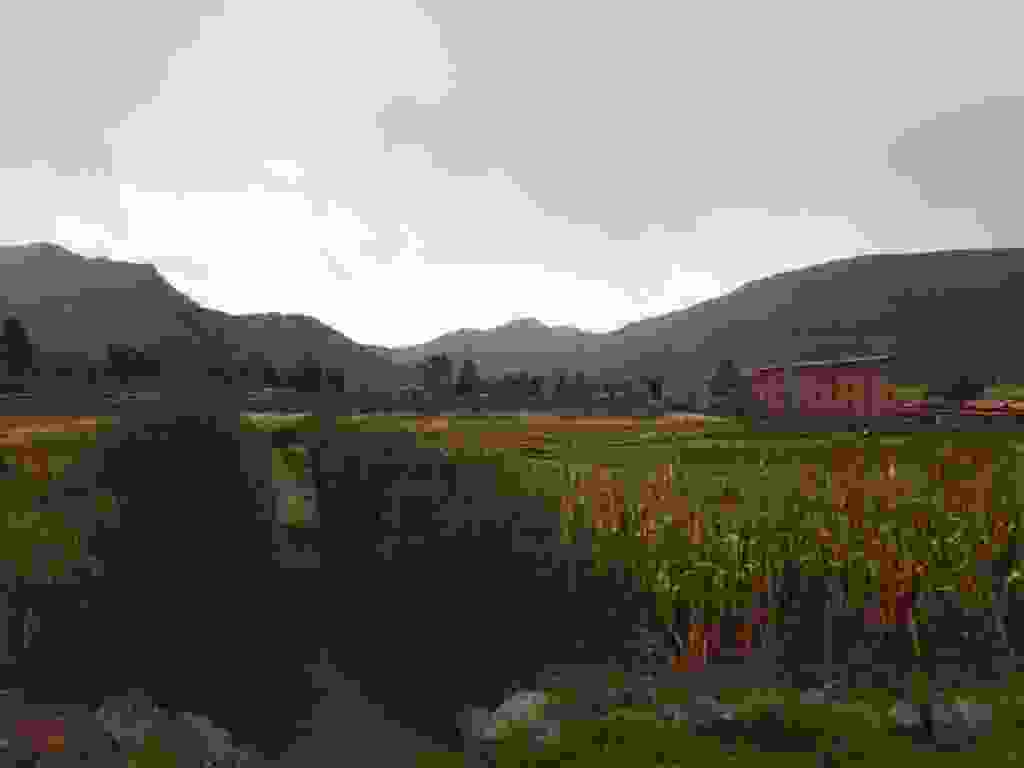
\includegraphics[width=\mywidth]{../wp-content/uploads/2015/05/P5154086-1024x768.jpg} \end{center}

 

 

\begin{center} 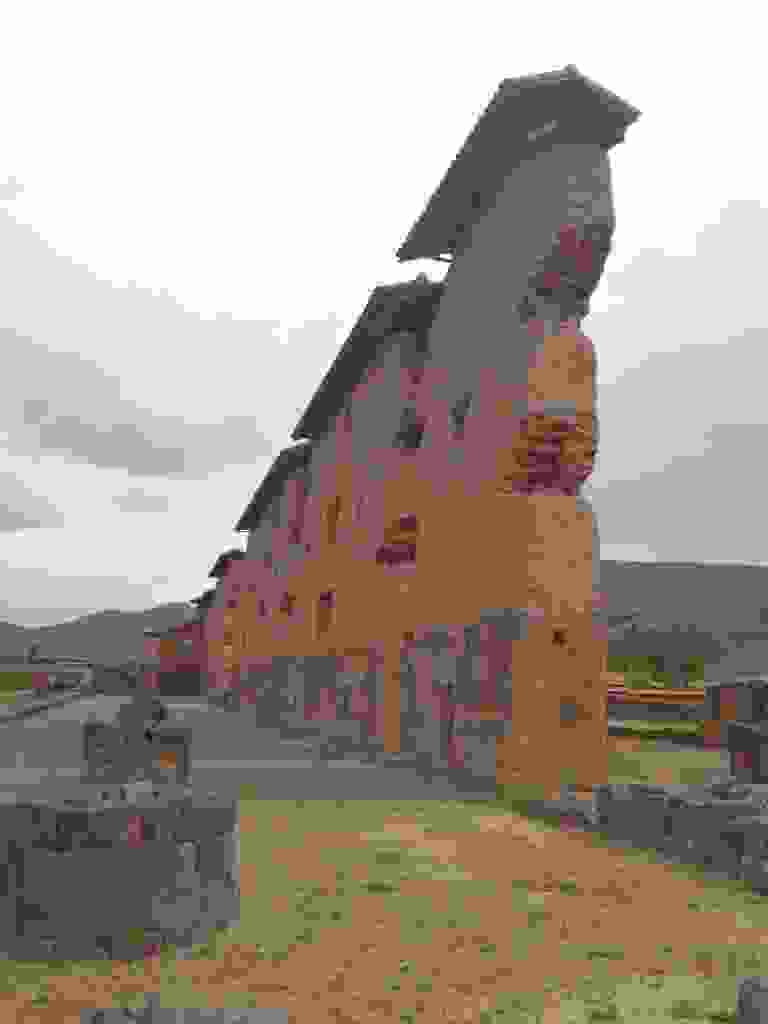
\includegraphics[width=\mywidth]{../wp-content/uploads/2015/05/P5154076-768x1024.jpg} \end{center}

 

 

\begin{center} 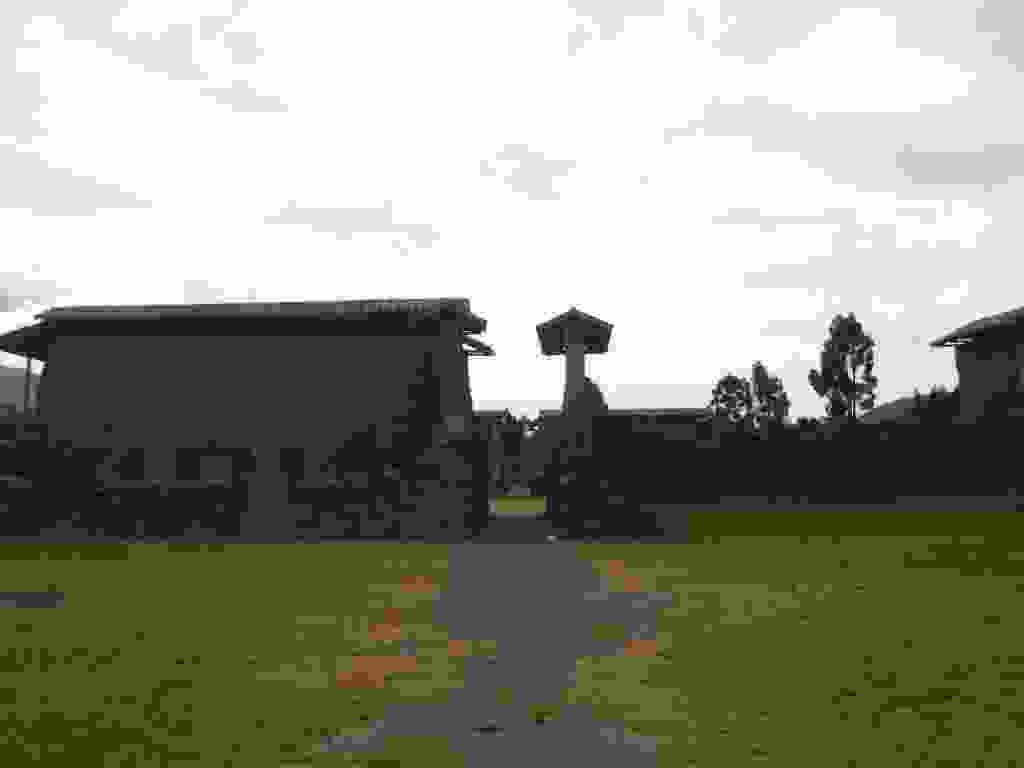
\includegraphics[width=\mywidth]{../wp-content/uploads/2015/05/P5154079-1024x768.jpg} \end{center}

 

 

\begin{center} 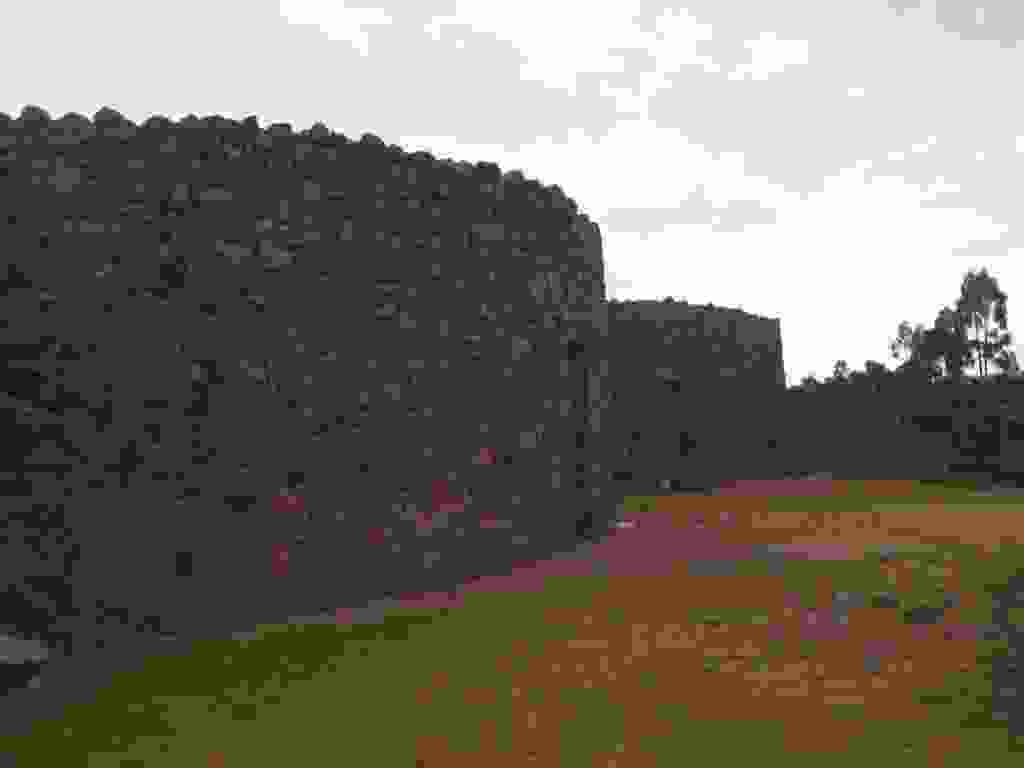
\includegraphics[width=\mywidth]{../wp-content/uploads/2015/05/P5154080-1024x768.jpg} \end{center}

 

 Dans le village d´Andihuaylillas, une belle église. 

 

\begin{center} 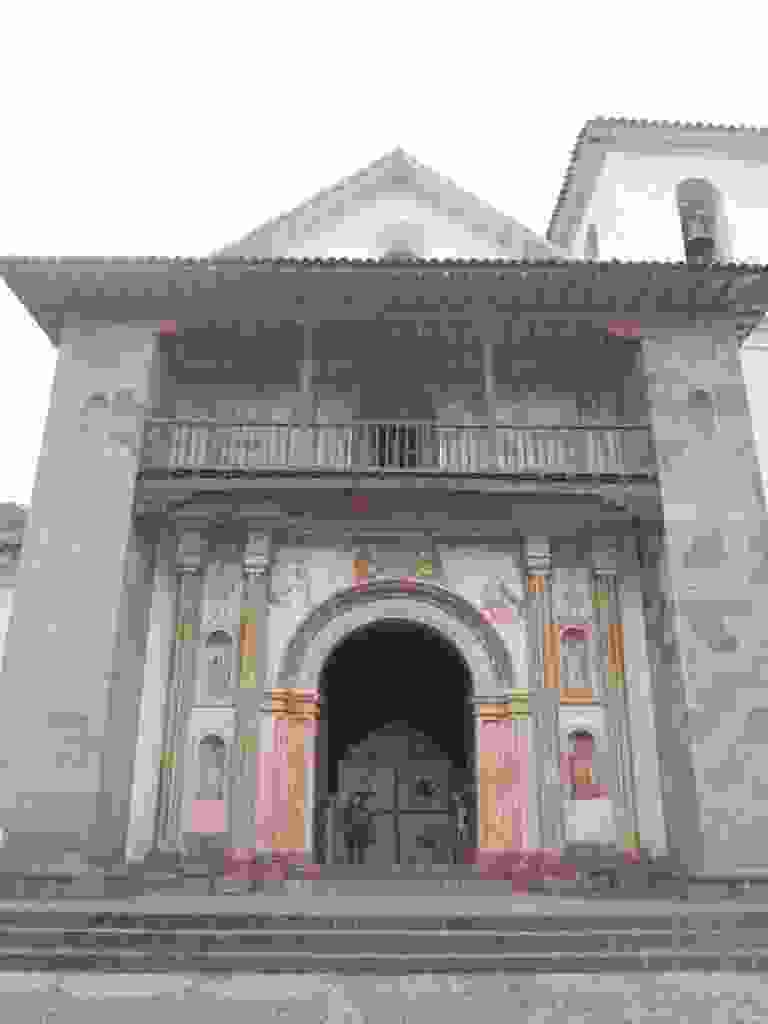
\includegraphics[width=\mywidth]{../wp-content/uploads/2015/05/P5164096-768x1024.jpg} \end{center}

 

 Au bord de la route une immense porte inca. 

 

\begin{center} 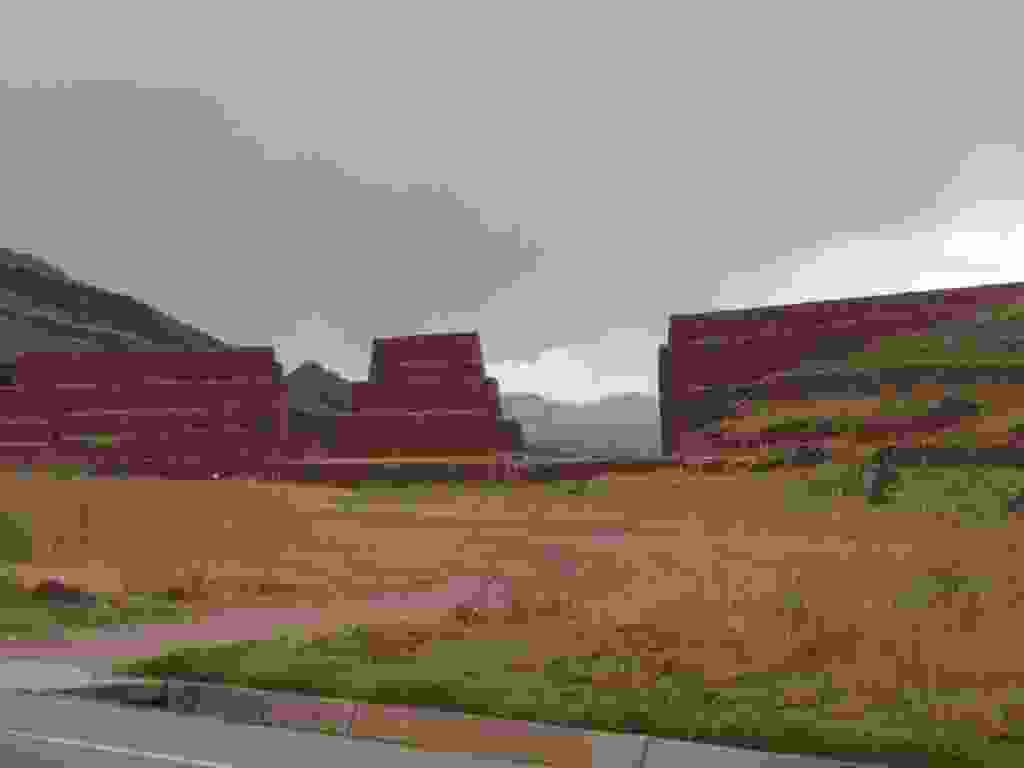
\includegraphics[width=\mywidth]{../wp-content/uploads/2015/05/P5164098-1024x768.jpg} \end{center}

 

 Puis le site pré-inca de Tiquillaka. 

 

\begin{center} 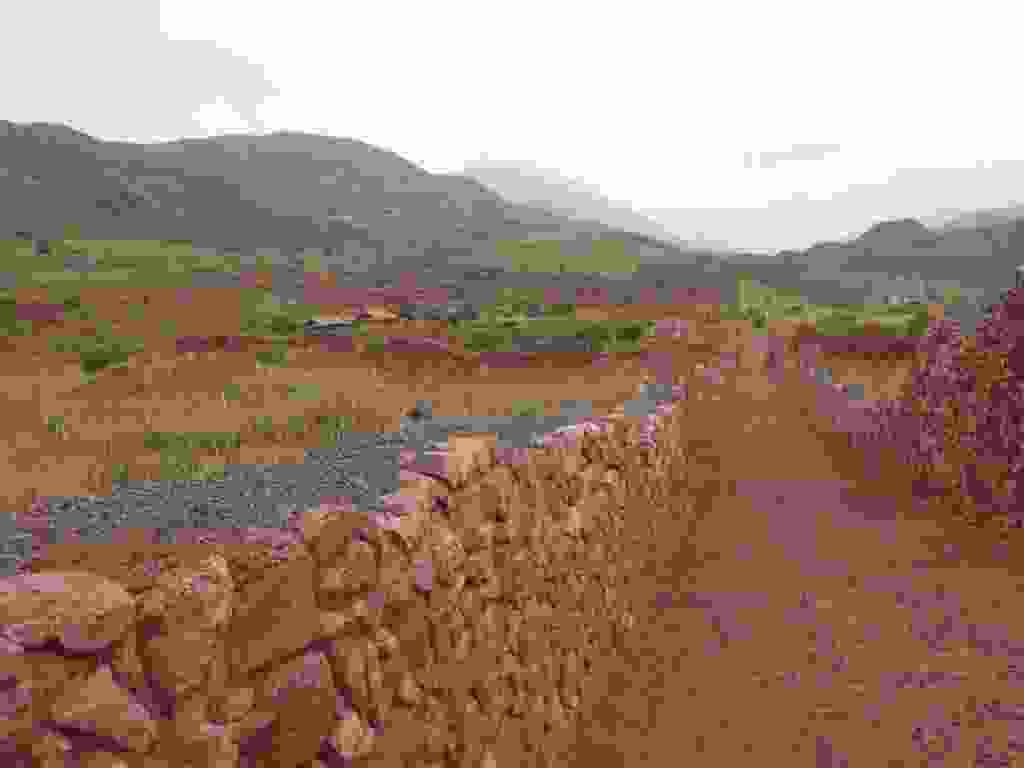
\includegraphics[width=\mywidth]{../wp-content/uploads/2015/05/P5164109-1024x768.jpg} \end{center}

 

 

\begin{center} 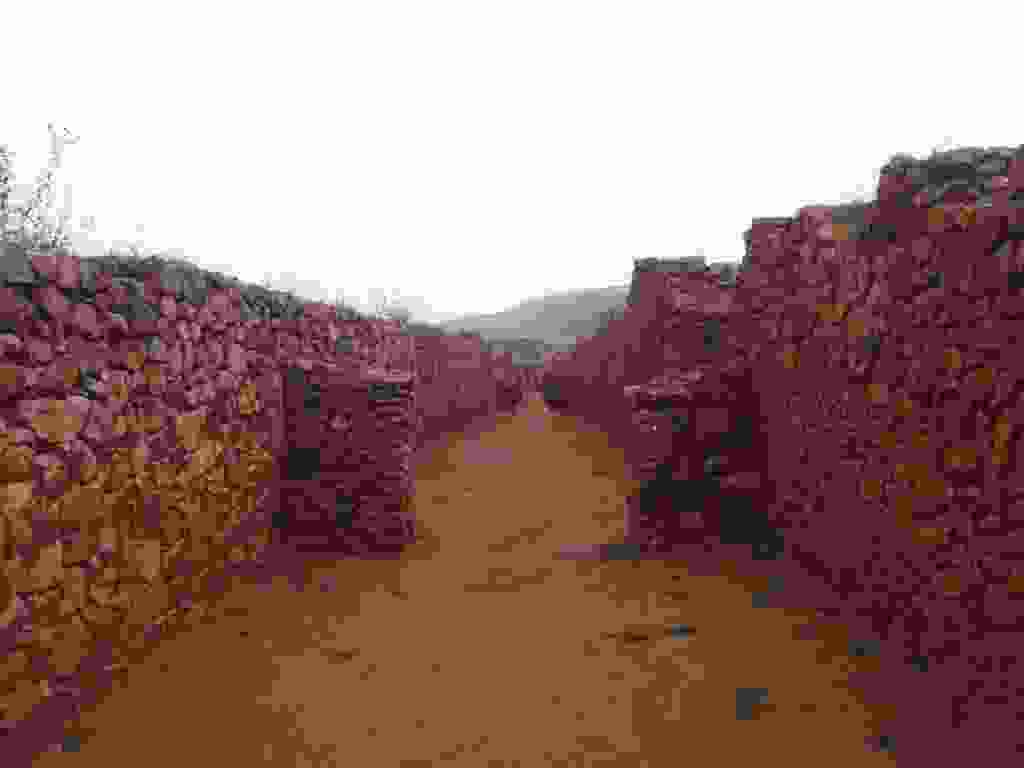
\includegraphics[width=\mywidth]{../wp-content/uploads/2015/05/P5164105-1024x768.jpg} \end{center}

 

 

\begin{center} 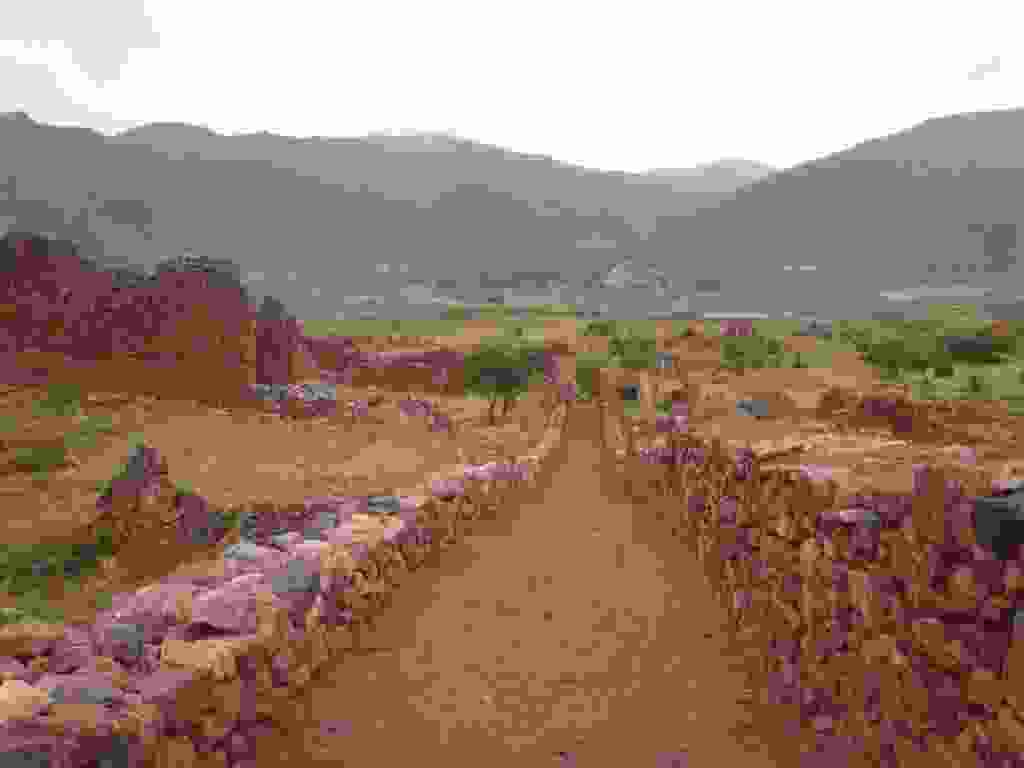
\includegraphics[width=\mywidth]{../wp-content/uploads/2015/05/P5164102-1024x768.jpg} \end{center}




 
 
